\documentclass{article}
\usepackage[swedish]{babel}	
\usepackage[utf8]{inputenc} 		
\usepackage{amsmath} 

\usepackage{fancyhdr}
\usepackage{lastpage}
\usepackage{lineno}
\usepackage{lmodern}
\usepackage[T1]{fontenc}
\usepackage[utf8]{inputenc}
\usepackage[swedish]{babel}
\usepackage{microtype}
\usepackage{systeme}
\usepackage{amsmath,amssymb,amsthm,mathrsfs,latexsym,tikz,url}
\usepackage{epigraph,graphicx}
%\usepackage{titlesec} %For formatting sections
\usepackage{listings}
\usepackage{listingsutf8}
\usepackage{color}
\usepackage{todonotes}
\presetkeys%
    {todonotes}%
    {inline,backgroundcolor=yellow}{}

\graphicspath{ {./}{./figures/} {images/}}
\DeclareGraphicsExtensions{.png,.pdf}

\definecolor{dkgreen}{rgb}{0,0.6,0}
\definecolor{gray}{rgb}{0.5,0.5,0.5}
\definecolor{mauve}{rgb}{0.58,0,0.82}

\lstset{frame=tb,
  language=Python,
  aboveskip=3mm,
  belowskip=3mm,
  showstringspaces=false,
  columns=flexible,
  basicstyle={\small\ttfamily},
  numbers=none,
  numberstyle=\tiny\color{gray},
  keywordstyle=\color{blue},
  commentstyle=\color{dkgreen},
  stringstyle=\color{mauve},
  breaklines=true,
  breakatwhitespace=true,
  tabsize=4
}


\setlength{\parindent}{0.0cm}
\setlength{\parskip}{0.1cm}



\begin{document}


\title{Lab 1 Machine Learning}
\author{Anton Stråhle \& Jan Alexandersson}
\maketitle 

\section*{Assignment 0}

\section*{Assignment 1}

\begin{center}
 \begin{tabular}{|c | c|} 
 \hline
 Dataset & Entropy  \\ [0.5ex] 
 \hline \hline
 MONK-1 & 1.0 \\ 
 %\hline
 MONK-2 & 0.9571174283 \\ 
 %\hline
 MONK-3 & 0.9998061328 \\ [1ex] 
 \hline
\end{tabular}
\end{center}


\section*{Assignment 2}

\section*{Assignment 3}

\begin{center}
 \begin{tabular}{|c | c c c c c c |} 
 \hline
 Dataset & A1 & A2 & A3 & A4 & A5 & A6 \\ [0.5ex] 
 \hline \hline
 MONK-1 & 0.07527 & 0.00584 & 0.00471 & 0.02631 & \textcolor{blue}{\textbf{0.28703}} & 0.00076 \\ 
 %\hline
 MONK-2 & 0.00376 & 0.00246 & 0.00106 & 0.01566 & \textcolor{blue}{\textbf{0.01728}} & 0.00625 \\ 
 %\hline
 MONK-3 & 0.00712 & \textcolor{blue}{\textbf{0.29374}} & 0.00083 & 0.00289 & 0.25591 & 0.00708  \\ [1ex] 
 \hline
\end{tabular}
\end{center}


\section*{Assignment 4}

\section*{Assignment 5}


Run the code below for MONK-1 and MONK-3 and their respective testdata to obtain a sample which we can 
compute the mean and variance on.

\begin{lstlisting}
def prune(data, test):
	pruned_trees_fraction = []
	for frac in fraction:
		train, val = partition(data, frac)
		t = d.buildTree(train, m.attributes)
		all_pruned = d.allPruned(t)
		
		#I suppose t is included in all_pruned
		best_tree_perf = 0
		for t in all_pruned:
			candidate_perf = d.check(t,val)
			if best_tree_perf < candidate_perf:
				best_tree_perf = candidate_perf
				best_tree = t
		
		pruned_trees_fraction.append(1-d.check(best_tree, test))
	return pruned_trees_fraction
\end{lstlisting}


\begin{center}
 \begin{tabular}{|c | c | c |} 
 \hline
 Dataset & Error(Train) &  Error(Test) \\ [0.5ex] 
 \hline \hline
 MONK-1 & 0.0 & 0.1713 \\ 
 %\hline
 MONK-2 & 0.0 & 0.30787 \\ 
 %\hline
 MONK-3 & 0.0 & 0.05556  \\ [1ex] 
 \hline
\end{tabular}
\end{center}


\section*{Assignment 6}

\section*{Assignment 7}

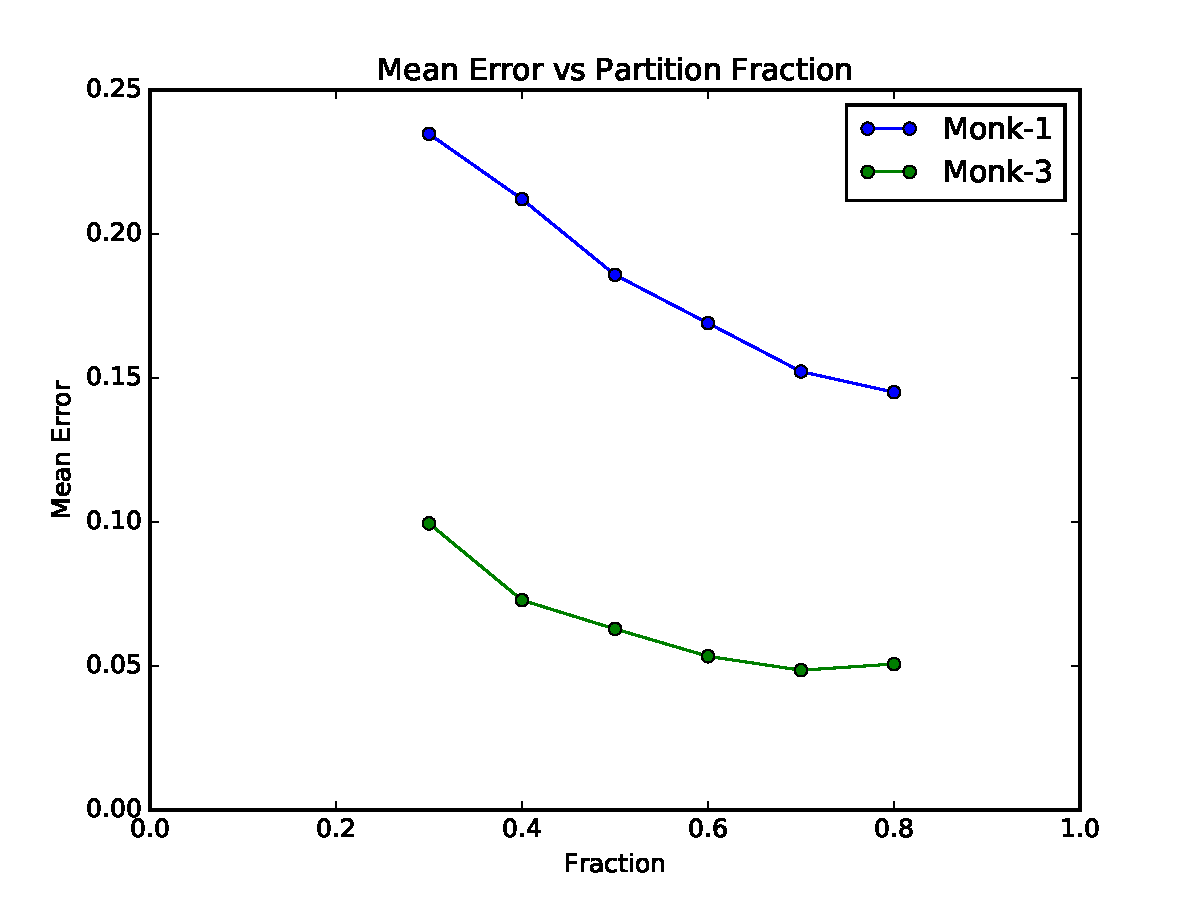
\includegraphics[width = 12cm]{figure_1.pdf}

\begin{center}
 \begin{tabular}{|c c c c c c c|} 
 \hline
 Fraction = & 0.3 & 0.4 & 0.5 & 0.6 & 0.7 & 0.8  \\ [0.5ex] 
 \hline 
 MONK-1 Sd \vline & 0.0436 & 0.0405 & 0.0409 & 0.0432 & 0.0415 & 0.0383 \\ 
 \hline
 MONK-3 Sd  \vline & 0.0578 & 0.0421 & 0.0378 & 0.0322 & 0.0284 & 0.0298 \\ [1ex] 
 \hline
\end{tabular}
\end{center}




\end{document}

